% Resultados propios C1 revisión 01; exportación auditada de EnergyPlus.
\clearpage
\subsection{Resultados preliminares del escenario pasivo C1}
\label{sec:c1-resultados}
La simulación anual de C1 reduce la demanda total de enfriamiento de 84.759,41 a 83.103,76 kWh térmicos, una diferencia de 1.655,65 kWh y una reducción del 1,95\,\% respecto al caso base. Esta magnitud incluye enfriamiento sensible y latente; no representa consumo eléctrico. La tabla~\ref{tab:c1-anual} conserva las 25 zonas con resultados de enfriamiento, incluidas aquellas con demanda nula.

\begin{table}[H]
\centering
\caption{Demanda anual de enfriamiento total por zona: caso base y C1.}
\label{tab:c1-anual}
{\fontsize{9}{11}\selectfont
\begin{tabular}{lrrrr}
\toprule
Zona & CB (kWh) & C1 (kWh) & C1 $-$ CB (kWh) & Variación \\
\midrule
PB-ASC & 0,00 & 0,00 & 0,00 & --- \\
PB-BA-01 & 0,00 & 0,00 & 0,00 & --- \\
PB-BO-01 & 0,00 & 0,00 & 0,00 & --- \\
PB-ES-01 & 0,00 & 0,00 & 0,00 & --- \\
PB-OF-01 & 2.800,60 & 2.639,71 & \textcolor[HTML]{2A9D8F}{-160,89} & \textcolor[HTML]{2A9D8F}{-5,74\,\%} \\
PB-OF-02 & 2.371,54 & 2.273,69 & \textcolor[HTML]{2A9D8F}{-97,85} & \textcolor[HTML]{2A9D8F}{-4,13\,\%} \\
PB-OF-03 & 3.062,20 & 2.984,56 & \textcolor[HTML]{2A9D8F}{-77,64} & \textcolor[HTML]{2A9D8F}{-2,54\,\%} \\
PB-RE-01 & 0,00 & 0,00 & 0,00 & --- \\
PB-SE-01 & 11.810,79 & 11.730,71 & \textcolor[HTML]{2A9D8F}{-80,08} & \textcolor[HTML]{2A9D8F}{-0,68\,\%} \\
1PA-BA-01 & 0,00 & 0,00 & 0,00 & --- \\
1PA-BA-02 & 0,00 & 0,00 & 0,00 & --- \\
1PA-DC & 40.196,11 & 40.147,08 & \textcolor[HTML]{2A9D8F}{-49,03} & \textcolor[HTML]{2A9D8F}{-0,12\,\%} \\
1PA-ES & 0,00 & 0,00 & 0,00 & --- \\
1PA-OF-01 & 4.447,65 & 3.948,92 & \textcolor[HTML]{2A9D8F}{-498,73} & \textcolor[HTML]{2A9D8F}{-11,21\,\%} \\
1PA-OF-02 & 2.967,62 & 2.837,18 & \textcolor[HTML]{2A9D8F}{-130,43} & \textcolor[HTML]{2A9D8F}{-4,40\,\%} \\
1PA-OF-03 & 4.500,53 & 4.059,70 & \textcolor[HTML]{2A9D8F}{-440,83} & \textcolor[HTML]{2A9D8F}{-9,80\,\%} \\
1PA-PAS & 0,00 & 0,00 & 0,00 & --- \\
1PA-SR & 3.053,31 & 3.014,99 & \textcolor[HTML]{2A9D8F}{-38,32} & \textcolor[HTML]{2A9D8F}{-1,25\,\%} \\
1PA-ASC & 0,00 & 0,00 & 0,00 & --- \\
2PA-BA-01 & 0,00 & 0,00 & 0,00 & --- \\
2PA-CAF & 2.642,02 & 2.638,45 & \textcolor[HTML]{2A9D8F}{-3,57} & \textcolor[HTML]{2A9D8F}{-0,14\,\%} \\
2PA-ES & 0,00 & 0,00 & 0,00 & --- \\
2PA-PAS & 0,00 & 0,00 & 0,00 & --- \\
2PA-SUM & 6.907,04 & 6.828,77 & \textcolor[HTML]{2A9D8F}{-78,27} & \textcolor[HTML]{2A9D8F}{-1,13\,\%} \\
2PA-ASC & 0,00 & 0,00 & 0,00 & --- \\
\midrule
\textbf{Total} & \textbf{84.759,41} & \textbf{83.103,76} & \textbf{$-$1.655,65} & \textbf{$-$1,95\,\%} \\
\bottomrule
\end{tabular}}
\fuente{Elaboración propia con resultados horarios de EnergyPlus, CB revisión 09 y C1 revisión 01, año de simulación 2025. Unidades térmicas. El guion indica una variación porcentual indefinida porque CB es cero.}
\end{table}

\clearpage
\subsubsection{Variación mensual por zona}
La figura~\ref{fig:c1-matriz-resultados} muestra que la respuesta del paquete varía durante el año. Algunas oficinas presentan aumentos de demanda entre enero y mayo, mientras que las reducciones son más pronunciadas en los meses posteriores. Los porcentajes comparan cada zona y mes con su propio valor base; no deben promediarse para obtener el ahorro anual del edificio.
\begin{figure}[H]
\centering
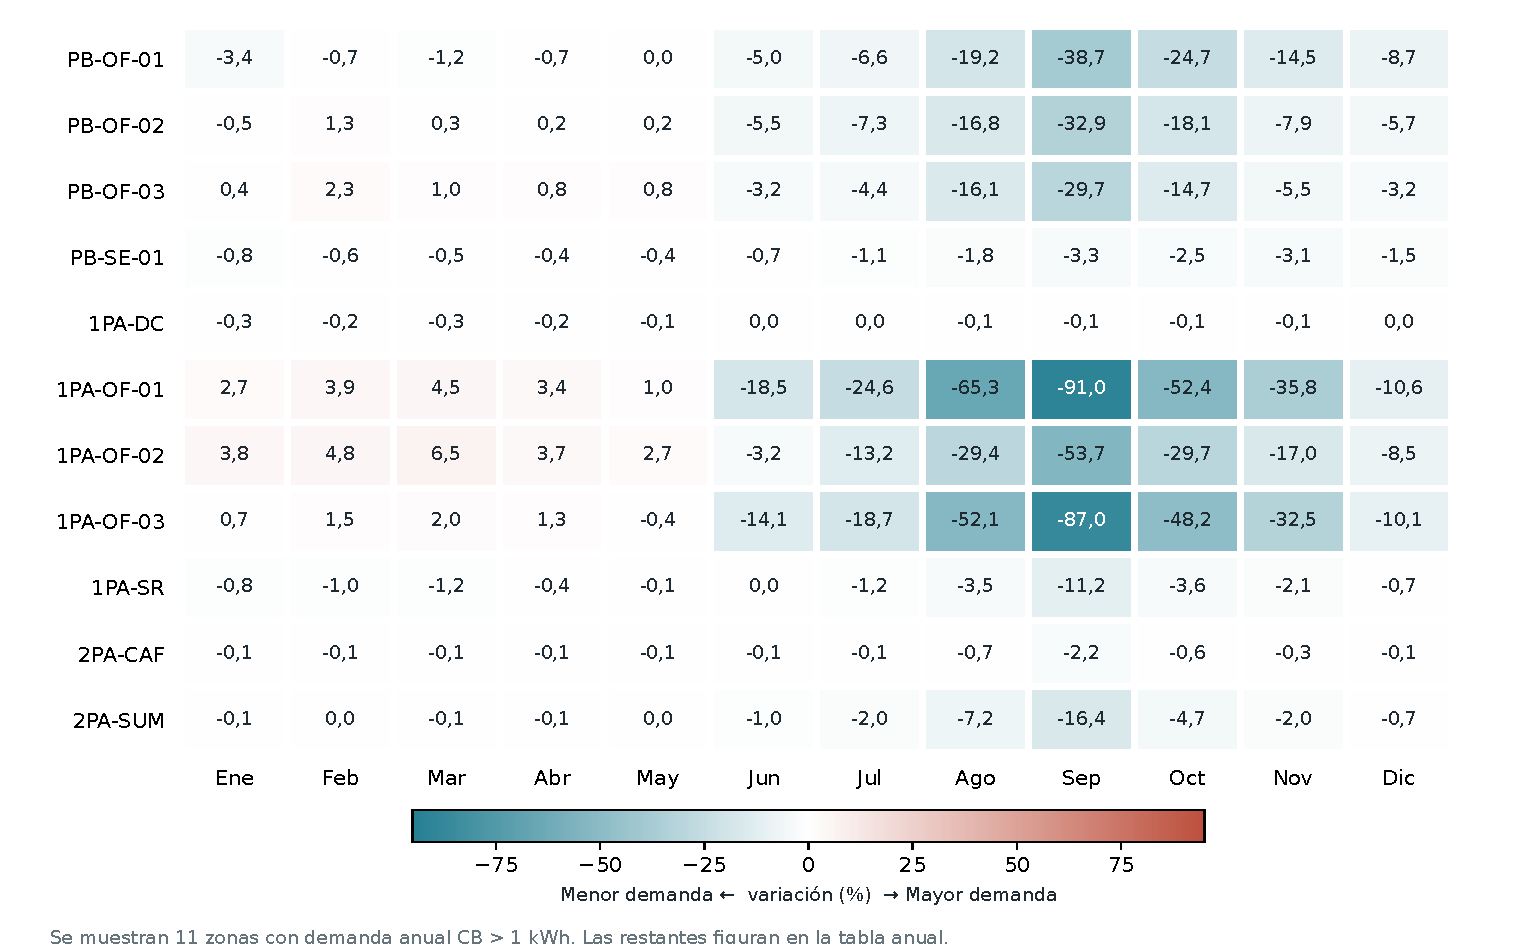
\includegraphics[width=\textwidth]{figuras/c1/02-matriz-mensual.pdf}
\caption{Variación porcentual mensual de la demanda de enfriamiento de C1 respecto al caso base.}
\label{fig:c1-matriz-resultados}
\fuente{Elaboración propia con resultados de EnergyPlus. Se muestran las 11 zonas con demanda anual base superior a 1 kWh. Turquesa: reducción; naranja: incremento. Variación = 100 $\times$ (C1 $-$ CB) / CB.}
\end{figure}

La reducción anual es preliminar. La corrida concluyó con 318 advertencias y ningún error severo, el mismo total de advertencias del CB. Esto acredita la finalización del cálculo, pero no resuelve los pendientes de entradas físicas, red de aire, confort ocupado e iluminación.

\clearpage
\subsubsection{Respuesta de las oficinas intervenidas}
Las seis oficinas presentan menor demanda anual en C1 (figura~\ref{fig:c1-oficinas-resultados}). La reducción oscila entre el 2,54\,\% en PB-OF-03 y el 11,21\,\% en 1PA-OF-01. Las conexiones representan pares de resultados de una misma oficina y no trayectorias temporales ni flujos de aire.
\begin{figure}[H]
\centering
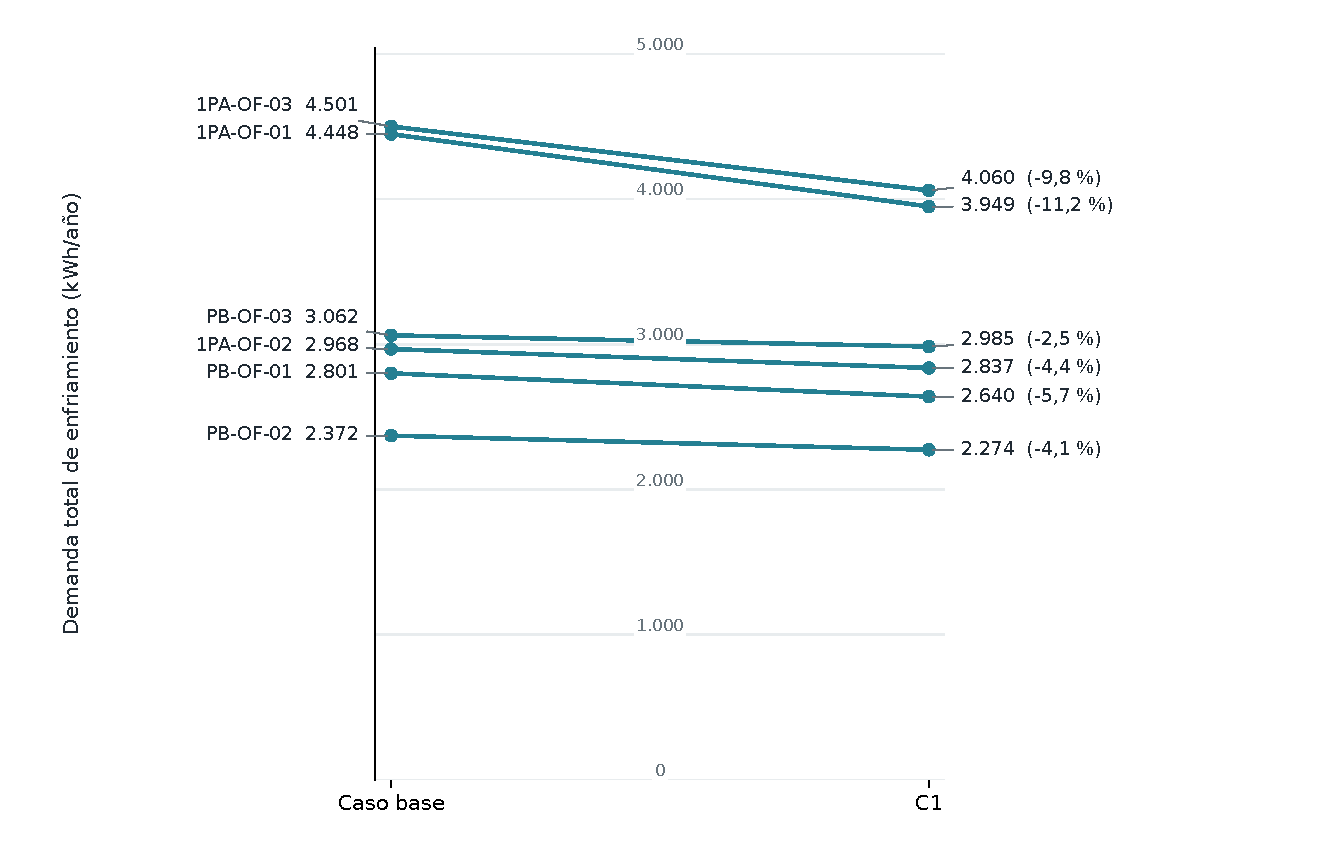
\includegraphics[width=\textwidth]{figuras/c1/03-cambio-oficinas.pdf}
\caption{Comparación de la demanda anual total de enfriamiento en las seis oficinas intervenidas.}
\label{fig:c1-oficinas-resultados}
\fuente{Elaboración propia con resultados de EnergyPlus, CB revisión 09 y C1 revisión 01. Valores en kWh térmicos por año; porcentajes referidos al CB de cada oficina.}
\end{figure}

La simulación conjunta no permite atribuir una fracción del ahorro a cada estrategia por separado. Para ello se requieren ensayos independientes de protección solar, apertura y control. Además, la disminución de demanda debe contrastarse con temperaturas durante la ocupación para descartar que responda a una reducción del servicio de refrigeración acompañada de menor confort.

\clearpage
\subsubsection{Distribución de aumentos y reducciones}
La figura~\ref{fig:c1-puntos-resultados} contabiliza las zonas con aumento, reducción o cambio no apreciable de demanda en cada mes. Cada punto tiene el mismo peso y representa una zona; por tanto, el número de puntos no expresa el volumen de energía ahorrada.
\begin{figure}[H]
\centering
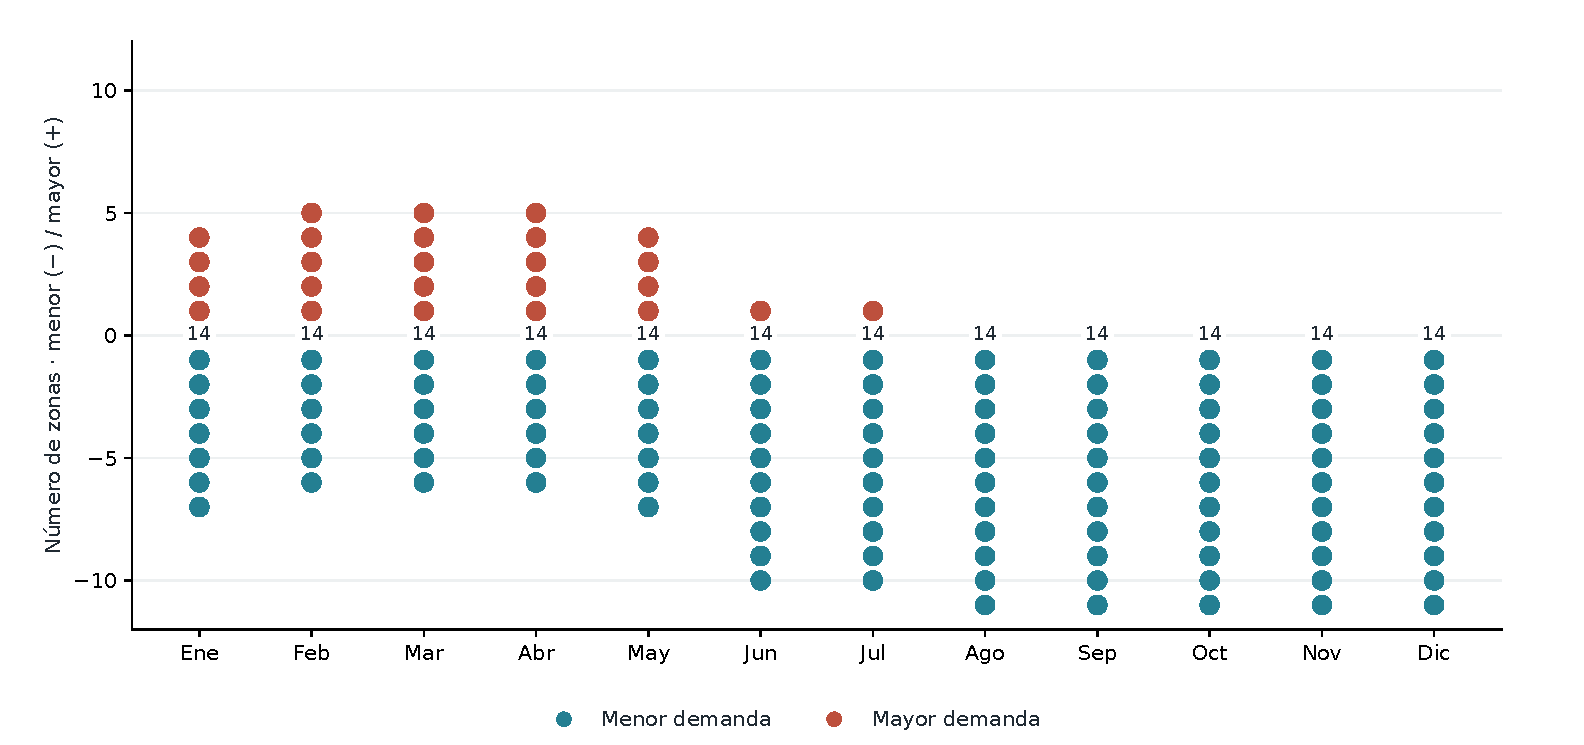
\includegraphics[width=\textwidth]{figuras/c1/04-zonas-por-mes.pdf}
\caption{Número de zonas con mayor y menor demanda mensual de enfriamiento en C1.}
\label{fig:c1-puntos-resultados}
\fuente{Elaboración propia con resultados de EnergyPlus. Base constante: 25 zonas con resultado de enfriamiento. La cifra sobre el eje cero identifica cambios de magnitud menor o igual a 0,1 kWh por mes; es una tolerancia de lectura, no un umbral normativo.}
\end{figure}

La integración de las potencias medias horarias se contrastó con los valores del periodo anual del archivo de resultados. Las tablas conservan la precisión original en los archivos CSV; los valores publicados se redondean para facilitar su lectura. C2 y C3 se presentan a continuación con resultados de sus propias corridas anuales.
\clearpage
